%
%  Allocating optional modules to University of York
%  students using constrained optimisation
%
%  BSc Computer Science/Maths final-year dissertation
%
%  Created by Alex Muller on 2011-10-10.
%  Copyright (c) 2011 Alex Muller. All rights reserved.
%
\documentclass[draft]{scrartcl}
% article, report, scrartcl, uoy_cs/UoYCSproject ?

\usepackage[utf8]{inputenc} % Use utf-8 encoding for foreign characters

% Pages and margins
\usepackage{fullpage}
\usepackage[top=2cm, bottom=4cm, left=2cm, right=2cm]{geometry}

\setlength{\parskip}{1ex plus 0.5ex minus 0.2ex}
% \addtolength{\parskip}{\baselineskip}
% \usepackage{parskip}

% Running Headers and footers
%\usepackage{fancyhdr}

% Multipart figures
%\usepackage{subfigure}

% More symbols
%\usepackage{amsmath,amssymb,latexsym}

\usepackage{boxedminipage} % Surround parts of graphics with box
\usepackage{lastpage} % Number of pages

\usepackage{xcolor} % Syntax highlighting etc
\definecolor{light-gray}{gray}{0.5}
\definecolor{yorkblue}{RGB}{0,38,99}
\definecolor{yorkgreen}{RGB}{24,69,59}

% Listings package for including code
\usepackage{listings}
\lstset{
  basicstyle = \ttfamily\footnotesize,
  % keywordstyle = \color{blue},
  % commentstyle = \color{red},
  numbers = left,
  numberstyle = \tiny,
  stepnumber = 20,
  numbersep = 12pt,
  frame = single,
  rulecolor = \color{light-gray},
}
\lstloadlanguages{HTML}

% This is now the recommended way for checking for PDFLaTeX:
\usepackage{ifpdf}

\ifpdf
\usepackage[pdftex]{graphicx}
\else
\usepackage{graphicx}
\fi

\ifpdf
\usepackage[pdftex]{hyperref}
\else
\usepackage{url}
\fi

\ifpdf
\usepackage{pdflscape}
\else
\usepackage{lscape}
\fi

\usepackage{ifdraft}

% Entity-relationship diagrams
\usepackage{libs/tikz-er2}

% Glossary
\usepackage{glossaries}
\makeglossaries
% Entries

% \newacronym[\glsshortpluralkey=cas,\glslongpluralkey=contrived
% acronyms]{aca}{aca}{a contrived acronym}

\newglossaryentry{itservices}{
  name = {IT Services},
  description = {
    is a support service that, ``together with the Library and Archives, forms
    the Information Directorate" at the University of York. It is responsible
    for, among other things, computer hardware and software, infrastructure
    and web services at the University}
}

\newglossaryentry{sits}{
  name = {SITS},
  description = {
    (Strategic Information Technology Services) is a piece of software
    manufactured by Tribal Group plc. It acts as the University of York's
    \gls{mis}, a database used to store staff and student details, including
    information on which modules are available}
}

\newglossaryentry{post}{
  name = {\texttt{POST}},
  description = {
    is an HTTP request method that allows web browsers to send data to a web
    server as part of the request body. \texttt{POST} requests are typically
    used for submitting forms or uploading files on the web},
  sort = {POST}
}

\newglossaryentry{mvc}{
  name = {model-view-controller},
  description = {
    is a software development pattern by which the presentation, data and
    logic are all separated in the application code}
}

\newglossaryentry{aso}{
  name = {Academic Support Office},
  description = {
    is an administrative office at the University of York that is responsible
    for improving processes around teaching and education. This final-year
    project was undertaken at the request of the Academic Support Office}
}

\newglossaryentry{ssdt}{
  name = {Student Systems Development Team},
  description = {
    is a team at the University of York responsible for the management of
    student data}
}

\newglossaryentry{routecode}{
  name = {route code},
  description = {
    is an identifier used by the University of York to indicate which specific
    course a student is taking. For example, UBENGAHIS3 is a route code
    referring to a three-year undergraduate History and English course}
}

\newglossaryentry{stage}{
  name = {stage},
  description = {
    is the University of York terminology for a student's current year of
    study}
}

% Acronyms

\newacronym{oscon}{OSCON}{The O'Reilly Open Source Convention}
\newacronym{dbms}{DBMS}{database management system}
\newacronym{html}{HTML}{HyperText Markup Language}
\newacronym{sso}{SSO}{single sign-on}
\newacronym{mis}{MIS}{management information system}
\newacronym{jsp}{JSP}{JavaServer Pages}
\newacronym{sql}{SQL}{structured query language}
\newacronym{yusu}{YUSU}{University of York Students' Union}
\newacronym{vpn}{VPN}{virtual private network}
\newacronym{kiss}{KISS}{keep it simple, stupid}
\newacronym{crud}{CRUD}{create, read, update and delete}
\newacronym{nda}{NDA}{non-disclosure agreement}
\newacronym{nss}{NSS}{National Student Survey}
\newacronym{owasp}{OWASP}{Open Web Application Security Project}
\newacronym{senda}{SENDA}{Special Educational Needs and Disabilities Act}
\newacronym{utc}{UTC}{University Teaching Comittee}
\newacronym{vm}{VM}{virtual machine}


% Title page stuff

\def\paperauthor{Alexander Muller}
\def\papertitle{Allocating optional modules to University of York students
using constrained optimisation}

\title{\papertitle}
\author{\paperauthor}
\date{\today}

% Properties

\hypersetup
{
    pdfauthor={\paperauthor},
    pdfsubject={A final-year BSc Computer Science project to allocate
      university modules},
    pdftitle={\papertitle},
    pdfkeywords={york, computer science, webapp, university, module,
      allocation}
}

\begin{document}

\ifpdf
\DeclareGraphicsExtensions{.pdf, .jpg, .tif}
\else
\DeclareGraphicsExtensions{.eps, .jpg}
\fi

\maketitle

This is the report for a Bachelor of Science final-year project in Computer
Science and Mathematics at the University of York. The project was supervised
by Dr James Cussens, Senior Lecturer in the Artifical Intelligence Group,
Department of Computer Science.

This report is 8,300 words, as counted by running \texttt{detex} and
\texttt{wc -w}. It is \pageref{LastPage} pages long.

% The limits are 35,000 words and 70 pages - neither limit may be exceeded.
% Other projects I've seen have been 12,000/60, 11,000/60, 21,000/71 etc

\ifoptiondraft{

  This report is a work-in-progress (a draft) compiled on \today.

  \medskip
  \textbf{Notes during report writing:}

  \begin{itemize}
    \item Not sure how to refer to people e.g. Laura
    \item Not sure how to refer to myself: ``project implementer'' or ``author''?
    \item Does the structure look ok?
    \item Should the title be changed? Something about a web application? 
  \end{itemize}

}

\clearpage

\begin{abstract}
  % Couple of paras. Not more than 200 words - this is 194.

  From their second year onwards, most students at the University of York can
  choose between two or more optional modules to tailor their academic career,
  in the hope that it will be more relevant, interesting and useful to them.
  
  Optional module allocation in some departments is handled using a paper form
  which must be returned to departmental administrators and processed
  manually. This project aims to design and implement a piece of web-based
  software that can be used by departments and students to allocate modules
  more fairly and with less administrative overhead.
  
  Allocating modules ``fairly'' involves understanding how staff and students
  view fair allocation, and translating that into a constrained optimisation
  problem solvable by a computer.
  
  The web application will be piloted by the Archaeology and History
  departments in Spring 2012 and, if successful, will be offered to all
  departments and maintained centrally by the University of York.
  
  This report discusses the choices made around the technology used, the
  development methodology and details relating to the allocation algorithm. It
  details specifics about the implementation, problems that arose and how they
  were mitigated, and some further work that could be carried out to improve
  the software.
\end{abstract}

\clearpage

\tableofcontents

\clearpage

\section{Statement of ethics}

% Informed consent

Those people volunteering to help with the project (interviewed during the
research stage) will at no point be put in a position of physical danger.
Consent will be obtained from all volunteers prior to their interview, and
volunteers' personal information will not be published or shared. A copy of
the consent form signed by all volunteers is given in
Appendix~\ref{sec:consent}.

% Do no harm

As far as the project author is aware, there are no immediate ethical issues
relating to the creation of the module allocation software.

% Confidentiality of data

The project steering group has noted that as a student, the author must not be
given access to any sensitive personal information. This includes, but is not
limited to, student names, email addresses and degree course information.
Development and testing of the software will be carried out with data that it
is in a similar form to real data held by the University. The University's
Data Protection Officer was consulted during the project, and their input is
discussed in Section~\ref{sec:dataprotection}.

\section{Introduction}

% The scope of the project, setting the scene for the remainder of the report.

This project is the result of requests by departments at the University of
York for more flexibility in the way they offer optional modules to
undergraduate students. The project is sponsored by University Teaching
Committee and is overseen in that regard by Laura Crossley of the \gls{aso}.

As well as being marked as an undergraduate project, the software will be
evaluated independently by Ms Crossley. If it is judged to provide sufficient
advantages over the current methods of module allocation, it may be
recommended that responsibility for the software is handed to \gls{itservices}.

\subsection{Report structure}

This section gives background information about the University of York
relevant to the project. Section~\ref{sec:requirements} discusses how the
project was run (with the help of administrative staff at the University) and
the requirements that were obtained from clients. Section~\ref{sec:research}
covers the research that was undertaken at the start of the project.
Section~\ref{sec:implementation} discusses the choices that were made during
the implementation of the software, and how it was tested before delivery.
Section~\ref{sec:furtherwork} describes ways in which the software could be
extended in the future. Section~\ref{sec:conclusions} gives the conclusions
drawn at the end of the project.

\subsection{The current state of module allocation}

% Refer to documents provided by Laura
% (1) At the University of York

Universities worldwide want to give their students the most interesting and
useful education possible, and one way this can be accomplished is by offering
flexibility in modules students can take. Generally speaking, a department
that offers a broad range of modules to choose from will see increased student
satisfaction with the course.

At the University of York, module allocation is dealt with at the departmental
level. Some departments make use of centrally offered software (eVision and
\gls{sits}), though several departments feel the software is not flexible
enough and continue to use paper-based forms that must be filled out and
returned to the departmental office. A smaller number of departments that have
the resources to implement their own system, such as Computer Science, have
written their own module choice and allocation software.

At some universities in the United Kingdom (for example, the Universities of
Warwick and Leeds), enrolement is completed online, on a first-come,
first-served basis.

% (2) Elsewhere around the world

\subsection{Web applications at the University of York}

% Student portal
% Timetabling gateway
% Google Apps for Education

The University is constantly improving the quality of web software available
to students and staff through providing updates to commercially obtained
software and employing developers to improve and maintain code written
in-house.

For the last few years, a \gls{sso} solution has been provided
centrally, using Shibboleth. This improves both user experience and security,
as users are encouraged to only ever enter their University username and
password into one screen, where the web address will always begin
\texttt{https://shib.york.ac.uk/}.

In September 2011, a new ``student portal'' was released, allowing students to
view personalised information relevant to them in one place. The application
was created by IT Services and was written in Java. Information on the student
portal is available at
\texttt{\href{https://www.york.ac.uk/students/about/}{www.york.ac.uk/students/about/}}.

For the beginning of the 2011--12 academic year, new timetabling software is in
use to give members of the University access to their complete timetable in
one location---something which has not been possible before.

In June 2012, the University will move all students to Google's Apps for
Education product for email and calendaring, one of the aims of which is to
improve the user experience dramatically over the current webmail software.

\section{Project management and requirements}
\label{sec:requirements}

The \gls{aso} identified pilot departments who would use the software to
allocate optional modules. A project steering group was formed consisting of
representatives from each of the departments (Archaeology and History),
administrative staff responsible for IT and timetabling, and the project
author and supervisor. The project steering group consists of:

\begin{itemize}
  \item Project implementer
  \item Project supervisor (Department of Computer Science)
  \item Project manager (\gls{aso})
  \item Head of Enterprise Systems (\gls{itservices})
  \item University Timetabling Officer (Campus Services)
  \item Chair of Board of Studies (Department of Archaeology)
  \item Departmental administrator (Department of Archaeology)
  \item Student representative (Department of Archaeology)
  \item Chair of Board of Studies (Department of History)
  \item Departmental administrator (Department of History)
  \item Student representative (Department of History)
\end{itemize}

Basic requirements for the project were given in the initial project
specification. At the first steering group meeting in May 2011 and later that
year this group reinforced and prioritised certain requirements. When the
project commenced, the requirements could be briefly summarised as:

\begin{quote}
  A system to allocate optional modules to university students. The system
  should be user-friendly and accessible via a web browser for both students
  and departmental staff. The system should provide benefits over the current
  paper-based method of allocating modules, such as:
  \begin{itemize}
    \item Reduce administrative overhead
    \item Improve student experience
    \item Increased level of fairness in module allocation
  \end{itemize}
\end{quote}

% \include{./sections/research}

\section{Research}
\label{sec:research}

% One or more review chapters, describing the research you did at the
% beginning of the project period.

As web application development is an area that requires solving problems in
many different areas of Computer Science, the research completed in this phase
of the project was wide-ranging.

\subsection{Development methodology}

% Agile?

% Prototyping

Zhang and Chung \cite{MODFM_2003} note that prototyping can be used to
reinforce client confidence as well as making better use of the time allocated
to development and implementation.

Bochicchio and Paiano \cite{PrototypingWebApplications_2000} note that
creating prototypes of web applications has several advantages.
The most relevant advantage for this project is that a mockup can be used to
get feedback from non-technical stakeholders such as the project manager and
the departmental contacts.

Prototypes can be defined as being low or high fidelity depending on how much
they are designed to resemble the final application. Low fidelity prototypes
can be creating using a marker pen and sheets of blank paper, whereas higher
fidelity prototypes may be coded to appear in a web browser and allow the user
to interact as they might with the final system.

% Iterative

Iterative development (also sometimes referred to as ``rapid application
development'') is a process by which the product is gradually improved through
trial and error. This differs from processes such as the waterfall method,
where testing follows implementation, which follows design, which follows
gathering of requirements. The key advantage of following an iterative
development process is that it allows far more flexibility than other
methodologies; it is common in software development that the requirements may
change or be refined over the duration of the project, and the development
process should be able to adapt as necessary \cite{kuniavsky2003userexperience}.

Kuniavsky points out that an iterative development process is especially
suitable for web applications, as prototypes can be created quickly. A low
fidelity prototype of a web application (which might consist of sketched
wireframes) can be created in a matter of minutes, while slightly higher
fidelity prototypes such as a simplified application front-end can be running
in a web browser within a day.

An iterative development process for this project might involve background
research with users (in the form of interviews), the creation of a prototype,
refining the user experience through more interviews, and repeating the
``prototype $\rightarrow$ interview $\rightarrow$ refine user experience
$\rightarrow$ interview'' cycle.

\subsection{Database design}

A \gls{dbms} is a piece of software that manages the
database, including providing the ability to add or edit records stored in the
database. The \gls{dbms} will be one of the more mature products used in the
creation of this system, with many having been available since the 1990s.

Relational databases are a common feature of web applications. We note
that the University of York already deploys MySQL and Oracle (both relational
model) database systems for its web applications and \gls{mis}.

When designing a database, Johnson \cite{DatabaseModelsLanguagesDesign} gives
several questions that he believes must be answered before a database can be
created:

\begin{itemize}
  \item What are the entities that need to be stored by the database?
  \item What are the relationships between these entities?
  \item What constraints are there on the database?
  \item What kind of queries will be written against this database?
\end{itemize}

All the questions above are relevant during the design of the database. While
the first three questions relate to the structure of the database, the final
question is especially important regarding database performance.

His method involves drawing an entity-relationship diagram (as the name
implies, this answers the first two questions in the form of a graph) and then
translating the E-R diagram into the database schema, which includes deciding
which fields will become primary and foreign keys. Any constraints (such as
minimum or maximum lengths of strings) can then be added depending on the DBMS
product being used.

\subsection{Maintainability and the future of the software}
\label{sec:maintainability}

As the software created for this project will have to be maintained by the
University's IT Services if it is evaluated as successful, care must be taken
to ensure that the application is implemented in the most extensible and
maintainable way possible.

Principles of good software engineering apply equally to web applications as
to any other software project. There are several basic methods recommended by
Green and Ledgard \cite{Green:2011:CGF:2063166.2063168} for writing readable
and maintainable code. Their recommendations are designed around the
maintainer of the software having to do less work to understand the purpose of
a given piece of code. The recommendations could be summarised as:

\begin{itemize}
  \item Align parts of the code (e.g. equal signs) vertically when it makes sense to
  \item Write lines no longer than approximately 70 characters, and use line breaks if necessary
  \item Use simple English and short names for things that will be referenced frequently
  \item Add blank space around operators (e.g. \texttt{3 + 2 = 5} rather than \texttt{3+2=5})
  \item Ident \texttt{if} statements to allow the reader to scan the code more easily
  \item Comment code when necessary, but comments are not a solution for bad code
\end{itemize}

They note that for any system that may have a long lifespan, every effort
should be taken to improve ``readability and maintainability''. A project that
will only be used for a short amount of time by the original author does not
require as much attention to maintainability as one which will last several
years and be maintained by several different programmers.

\subsection{Web application frameworks}

% Intro to (web) frameworks in general

A framework is a certain amount of reusable code that helps application
developers by reducing the complexity of common web operations. For example,
any moderately complex application will need to write user input to a data
store, and protecting against malicious input is an obvious concern when
executing code in a database.

Many frameworks include functions that write to the database on behalf of the
developer, and will automatically sanitise all input to prevent against
attacks. As every application written should sanitise user input, it is this
kind of repetitive action that frameworks help ease. A useful framework should
increase the amount of time that a developer can spend building the unique
parts of their application.

A key focus of \gls{mvc} frameworks is to separate the application logic from
the interface that is presented to the user. The term MVC splits the
application into three pieces; the model for structuring and imposing
constraints on the data, the controller for manipulating the data into a
usable format and the view for presenting the manipulated data to the end user
in an understandable way.

Parr \cite{Parr2004templateengines} makes the point that separating the model
from the view is something developers strive for, but often fail to achieve.
He provides some good examples of software development patterns that should
never be seen, such as including \gls{sql} statements anywhere except the
model -- and even then, the framework should provide a mapping between
application objects and database structure.

He cites maintainability as a reason to strictly separate the view from both
the controller and the model, and as maintability is a key focus of this
project (see Section~\ref{sec:maintability}) this is clearly important.


The way in which the web application framework for this project was chosen is
discussed in Section~\ref{sec:webframeworks}.

\subsection{Sensitive information and the Data Protection Act}
\label{sec:dataprotection}

% As noted in the Statement of ethics, we should discuss Charles' input here.

The software created for the purpose of this project will manipulate students'
personal data, and as such the University's Data Protection Officer was
consulted during the requirements gathering, design and implementation. He
provided input on how the software should comply with all relevant legislation
-- this section outlines his input and resulting actions taken.

\noindent{\textbf{Automated decision making}}

Under Section 12 (Part II) of the Data Protection Act 1998 c.29, an individual
can request that no automated decisions are made that affect that individual.

For the purposes of this project, departments must notify students that their
modules will be allocated automatically -- words to this effect were placed in
the departmental student handbooks for this academic year, and will be
reinforced by email when students are asked to choose their modules.

The project steering group decided that any student who requests that their
modules are allocated manually will be treated as an exception. However, the
departments noted that it would be very hard to ensure every student was
treated fairly when some were allocated using the software and others were
not.

It is expected that only a tiny proportion of students would make this
request, if any. As in previous years, students will of course have the right
to appeal their module allocation if they feel it is unfair.

The relevant legislation is available in full at
\url{http://www.legislation.gov.uk/ukpga/1998/29/section/12}.

\noindent{\textbf{Retaining a memory}}

If data about students is retained, it will need to be held in line with
University policies and a data retention policy will have to be created for
this system.

\noindent{\textbf{Transferring data between systems}}

The Data Protection Act requires any transfer of data between University
systems to be secure and accurate.

The only data transferred to \gls{sits} will be module allocation information
for each student. As this is entirely the purpose of collecting the data from
students in the first place, it was felt that no further work would be needed
to ensure compliance with the Act.

\noindent{\textbf{Compromise of student data}}

The Data Protection Officer notes that \emph{any} data input by students into the
system is ``their personal data'', and any compromise of this data would be a
breach of the Data Protection Act.

The project implementer will work with \gls{itservices} during the creation of
the software. They will ensure as far as they can that there are no security
issues in the software that would cause personal information to be compromised.

Furthermore, the software will be restricted by the University firewall so
that it can only be accessed by a person with a University of York username
and password. While this does not completely remove any issue, it will reduce
the impact of any security problems with the software.

\subsection{Online security}

Recently there has been increased public awareness of online security because
of exploits from groups such as ``Lulzsec''. Groups such as this have
exploited vulnerabilities and released sensitive information from
organisations such as Sony, the FBI, etc [reference required here].

While some of their attacks have involved social engineering, those is outside
the scope of this report. The research conducted here focuses solely on the
technical methods that should be used to prevent unwanted disclosure of
information.

[Todo: a basic overview of the OWASP top 10 vulnerabilities here]

\subsection{User testing}

Jakob Nielsen is a web usability expert who has been publishing articles on
his website, \url{http://www.useit.com/}, since 1995. In ``Why You Only Need to
Test with 5 Users'', Nielsen asserts that usability tests should be run for all
web projects, no matter how short the project timescale or limited the budget.
This is especially relevant for a project such as the module allocation
system, where the entire application must be developed in under six months and
there is no budget allocated. Nielsen's advice is to run a single usability
test with no more than five volunteers, and to run different tests if more
participants can be recruited. His reasoning is that iterative design with
testing after each iteration will uncover any problems unwittingly created
during the development process. Finally, Nielsen points out that distinct
groups of users need to be treated separately during user testing
\cite{nielsen2000fiveusers}.

Nielsen Norman Group, a company founded by Nielsen with Don Norman in 1998,
publishes reports on web usability. Among the 230 tips offered in one such
report \cite{nng2001tipsusability}, Molich describes how to conduct user
testing sessions. The bulk of his recommendations are around making the test
participant feel comfortable during the session; this involves reassuring them
that they are not being tested, telling them that they should simply perform
the tasks as though they were at home and making the first task simple to
allow the participant to gain confidence.

Cennydd Bowles and James Box work for a web design agency based in Brighton.
In ``Undercover User Experience Design'', Bowles and Box describe various
methods of usability testing with little time or budget. They give advice on
asking questions in an unbiased way, so as not to influence the test. Like
Nielsen, they advocate around five user tests, stating that even one is better
than none. The authors suggest recording video (or, failing that, audio) of
the interview as there will not be enough time to take notes during the
session.

Bowles and Box put forward another method of eliciting information from users,
namely the corridor test. This involves watching people use the current system
for a very short amount of time and observing any usability issues they
encounter. The primary advantage of this type of test is that it takes very
little time or effort on both the part of the participant and the researcher
\cite{bowles2011undercover}.

In a 1982 paper titled ``Pitfalls of user research, and some neglected areas''
\cite{brittain1982pitfalls}, J. M. Brittain sets out the different kinds of
study that can be carried out during the research phase of any project. These
are publishing a questionnaire or interviewing users, asking users for any
input they have regarding a system or service, and observing users while they
perform a task. One point made by Brittain is that user research is
occasionally too narrow-focused -- in his example, the library was focusing
``upon the demands users make for documents'' without necessarily considering
how users read the documents once they are in possession of them. In the case
of the web, one could argue that user research focuses too much on the
specific task of interest and not on how users browse the web from day-to-day
or what they generally use the web for.

User research (interviews with potential users or the distribution of
questionnaires) should take place before the design phase in order to create a
desirable product. Kuniavsky \cite{kuniavsky2003userexperience} describes a
``family and friends usability test'' that he claims provides immediate
feedback on a prototype with minimal preparation and time required from the
research participant.

His key points for conducting a usability study are:

\begin{enumerate}
  \item Define your application's audience and the goals they want to achieve
  \item Create scenarios that will help them accomplish their goals
  \item Find test participants
  \item Observe them while they play out the scenarios defined
\end{enumerate}

Kuniavsky reinforces Molich's point that the most important consideration
during a usability test is that the participant is comfortable; for example,
that they understand it is not they who are being tested, but the application.
He says that participants should be strongly encouraged to narrate their
thought process as they use the application, as this provides useful insight
to the researcher when they review the studies later.

\subsection{Usability}

% http://www.faqs.org/docs/artu/ch11s01.html
% http://en.wikipedia.org/wiki/Principle_of_least_astonishment

In the past, web applications would \gls{post} data to the web server when the
user clicked a submit button. Modern web applications, such as Google's Gmail
email service, make use of JavaScript and fast Internet connections to
automatically save data to the server while the user is working. Sandlund
\cite{sandlund2009websoftware} explains that by automatically saving data at
regular intervals, there is far less chance of data loss. However, it is
important to include an explicit ``Save'' button on an application that
auto-saves -- one can imagine the confusion and uncertainty caused if the user
is unaware that their data is being saved in the background.

\begin{lstlisting}[language=HTML]
<input type="submit">
\end{lstlisting}

During Sandlund's user testing, participants responded positively to the
application automatically saving data. However, Sandlund decided not to
include a submit button in his application, and he notes that some users found
the lack of an explicit save button ``a bit disturbing''.

\subsection{Performance testing}

If there's time...

\section{Development, implementation and testing}
\label{sec:implementation}

% Several chapters describing what you have done, focusing on the novel
% aspects of your own work.

After researching the areas noted in the previous section, the software was
researched, written and tested. This section describes how users helped
influence the design of the software during interviews, a discussion on web
frameworks, the visual appearance and other important factors for web
projects.

\subsection{Database structure}

We start with a table of entities:

\begin{tabular}{ l l }
  Student    & Student ID (key), name, course \\
  Allocation & Student ID (foreign key), module ID (foreign key) \\
  Module     & Module ID (key), department ID (foreign key), name, class size \\
  Department & Department ID (key), name \\
  Staff      & Staff ID (key), department ID (foreign key) \\
\end{tabular}

As relational databases are so popular and are supported in many of the
software frameworks we look at in Section~\ref{sec:webframeworks}, there is no
advantage to choosing a database model apart from relational.

Web frameworks abstract away anything related to a specific database product,
so the module allocation application can be written without regard for the
final database product that IT Services will use to deploy the application.

\subsubsection{Entity-relationship diagram}

Figure~\ref{er_diagram} is an entity-relationship diagram of the module
allocation system.

\usetikzlibrary{positioning}
\tikzstyle{every relationship} = [draw=black, fill=black!10, text=black]
\begin{landscape}
\begin{figure}
  \begin{tikzpicture}[node distance=8em]
    
    \node[entity] (student) {Student};
      \node[attribute] (studentid) [above=1cm of student] {\key{Identifier}} edge (student);
      \node[attribute] (routecode) [above left=1cm of student] {Route code} edge (student);
    
    \node[relationship] (makes) [below left of=student] {Makes} edge (student);
    
    \node[entity] (choice) [below of=makes] {Choice} edge (makes);
      \node[attribute] (rank) [left=1cm of choice] {Rank} edge (choice);
    
    \node[relationship] (given) [below right of=student] {Given} edge (student);
    
    \node[entity] (allocation) [below of=given] {Allocation} edge (given);
    
    \node[relationship] (allocof) [below of=allocation] {Of} edge (allocation);
    \node[relationship] (choiceof) [below of=choice] {Of} edge (choice);
    
    \node[entity] (moduleav) [below left of=allocof] {Module Availability};
      \node[attribute] (studentmin) [below left=0cm and 1cm of moduleav] {Student min} edge (moduleav);
      \node[attribute] (studentcap) [below left=1.2cm and 1cm of moduleav] {Student cap} edge (moduleav);

    \draw[link] (choiceof) |- node [pos=0.05, auto, swap] {} (moduleav);
    \draw[link] (allocof) |- node [pos=0.05, auto, swap] {} (moduleav);

  \end{tikzpicture}
  \caption{(Incomplete) Entity-relationship diagram for the module allocation system.}
  \label{er_diagram}
\end{figure}
\end{landscape}

% Helpful demo/test document

% \begin{landscape}
% \tikzstyle{every entity} = [top color=white, bottom color=blue!30, draw=blue!50!black!100]
% \tikzstyle{every attribute} = [top color=white, bottom color=yellow!20, draw=yellow, node distance=1cm]
% \begin{tikzpicture}[node distance=1.5cm, every edge/.style={link}]
%   \node[entity] (emp) {Employee};
%   \node[isa] (isa) [below=1cm of emp] {ISA} edge (emp);
%   \node[entity] (mec) [below left=1cm of isa] {Mechanic} edge (isa);
%   \node[entity] (sal) [below right=1cm of isa] {Salesman} edge (isa);      %%%%%%%%%%
%   \node[relationship] (does) [left=of mec] {Does} edge (mec);
%   \node[weak entity] (rep) [below=of does] {RepairJob} edge (does);
%   \node[ident relationship] (reps) [below=of rep] {Repairs} edge [total] (rep);
%   \node[entity] (car) [right=of reps] {Car} edge [<-] (reps);
%   \node[relationship] (buy) [below=of sal] {Buys};                         %%%%%%%%%%
%   \node[relationship] (sel) [right=of buy] {Sells};                        %%%%%%%%%%
%   % \node[derived attribute] (sval) [right=of sel] {Value} edge (sel);
%   \draw[link] (car.10) -| (buy) (buy) edge (sal);
%   \draw[link] (car.-10) -| (sel) (sel) |- (sal);
%   \node[entity] (cli) [below right=0.5cm and 3.7cm of car] {Client};
%   % \node[multi attribute] (cphone) [below right=of cli] {Phone} edge (cli);
%   \draw[link] (cli.70) |- node [pos=0.05, auto, swap] {buyer} (sel);
%   \draw[link] (cli.110) |- node [pos=0.05, auto] {seller} (buy);
% \end{tikzpicture}
% \end{landscape}


\subsection{User research}

In the weeks before implementation started, students and staff were
interviewed to understand more about their relationship with module
allocation. The chart in Figure~\ref{bowles_dualpurpose_chart} was originally
published by Bowles and Box and is incredibly relevant to this project.

The first user interviews (discussed in more detail in the following
subsections) consisted mostly of research; for example, discussing how module
allocation has worked in previous years. With this knowledge, a prototype
could be created. The later user sessions focused more on testing the
prototype with users to refine it and improve the user experience.

Screenshots of the three prototypes of the student interface used in testing
are given in Appendix~\ref{sec:prototypes}.

\begin{figure}
  \begin{center}
    \fbox{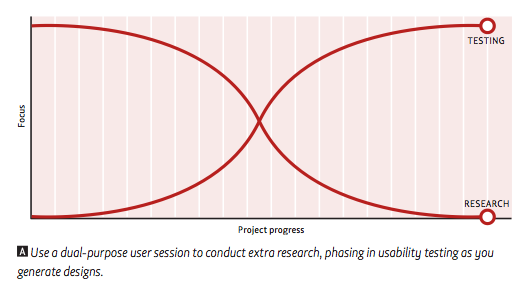
\includegraphics[width=120mm]{images/bowles_dualpurpose_testing.png}}
  \end{center}
  \caption{User session focus chart originally published in
    ``Undercover User Experience Design'', Bowles and Box \cite{bowles2011undercover}.}
  \label{bowles_dualpurpose_chart}
\end{figure}

\subsubsection{With students}

In the meetings with students, the questions asked predominantly revolved
around module allocation at the University of York; it was important to
understand how students feel about the current state of module allocation to
ensure that this system improves their experience.

Students were asked to use a mockup of the application written in \gls{html}
and the researcher observed them to discover the main sources of difficulty.
Students were asked how and where they access to web, to get an understanding
of the environments this application might be used in.

During the implementation phase of the project, focus groups organised by the
\gls{aso} were conducted with students from each of the pilot departments. The
project manager discussed with the students their current understanding of
module allocation, and their feelings on where it worked well and how it could
be improved. The project implementer tested several mockups of the student
interface by asking the students to visit hyperlinks. After the students had
the chance to use the mockups in a University computer classroom, they were
provided refreshments and took part in a discussion to gather their feedback.

In the History student focus group (eight students from 1st to 3rd year), it
was immediately clear that the two-column drag-and-drop layout
(Figure~\ref{prototype_student_2col}) was the easiest to use and related to
students' existing mental model most closely. As one student at the focus
group commented, this interface closely resembles the way in which the
\gls{yusu} website allows students to vote for sabbatical officers during
their annual elections. As students will already have some (however minimal)
experience with this kind of interface it makes sense to reuse ideas they are
used to.

Students were pleased with the simple drag-and-drop single column prototype,
but preferred the more explicit action of dragging from one side of the page
to the other. The weighting based system (dragging horizontal bars) was
unpopular with the History students; they commented that it would be
advantageous to have a simple system that all students can understand easily,
rather than one which may cause confusion -- especially when students are
preoccupied with making their module choices and do not want to think about
the way in which the system works.

In the Archaeology student focus group (six students from 1st to 3rd year),
similar concerns were raised about the second mockup. The students wondered
how the system would react if a student weighted only one or two modules
incredibly heavily and the remaining modules equally lightly. This is a
concern that would have to be discussed with the departments in depth and
communicated clearly to students in order to come up with a fair allocation.

The students again commented on the similarity between the \gls{yusu} website
and the second mockup, reinforcing the previous group's feedback that this
mockup was the best of the three.

With this group of students, it was easy to observe a common issue with
running focus groups. Two of the Archaeology students present were more
quiet than the others in the group and it was harder to get their opinions.
The solution in this case was to direct specific questions at those two
students, though obviously this was not ideal. If running the session again,
it would be advantageous to not include those students in the focus group
and instead gather their opinions without the other students present.

\subsubsection{With staff}

I also spoke to departmental administrators, who will be responsible for setting up
the system. We discussed:

\begin{itemize}
  \item The idea of ``fairness''
  \item The user interface
  \item Administration
\end{itemize}

% Discuss the results of the staff interviews

\subsection{Web application frameworks}
\label{sec:webframeworks}

% Justifying a framework for this project

While it is possible to build a web application without using a framework,
there is no advantage to rewriting basic operations for this project. If the
system needed to operate at a scale or speed far beyond what these frameworks
were capable of, it is likely that the software would have to be built from
scratch to meet those requirements.

With the limited amount of time allocated to development and implementation,
it is sensible to spend a small amount of time choosing a framework to allow
more time to implement the system.

%   Could reference the Gantt chart (if it's included) here.

\subsubsection{Framework language}

% The programming language

The most important consideration when choosing a framework is the language it
is written in, as this defines, among other things, how easy the software will
be to maintain in the future.

% ColdFusion ML
%   - http://www.york.ac.uk/communications/websites/content/programming/cms-integration/
% Java
% PHP
%   - http://www.york.ac.uk/it-services/facilities/web/php/

There are three languages used for most web development at the University of
York. \emph{ColdFusion Markup Language} (CFML) is a language for creating web pages,
the most popular commercial implementation of which is Adobe ColdFusion.
ColdFusion is used widely across the University, including in applications
such as the ``People Directory'' search tool (shown in
Figure~\ref{yorkacuk_directory_search}) and online account management
facilities. \emph{Java} was used in the creation of the new Student Portal. A
\emph{PHP} service is offered by the University for users to deploy their PHP
applications.

\begin{lstlisting}[language=HTML]
<cfparam name="attributes.userid" type="string" default="unknown">
<h1>Hello, world</h1>
<cfoutput>
  <p>Welcome, #HTMLEditFormat(attributes.userid)#.</p>
</cfoutput>
\end{lstlisting}

In a presentation at \gls{oscon} in 2007 \cite{raible2007javawebframeworks},
Matt Raible compared several web frameworks written in Java; JavaServer Faces
(JSF), Spring MVC, Stripes, Struts 2, Tapestry and Wicket.

While there are a wide variety of Java web application frameworks available,
the University of York has decided to use Spring, an open source framework
developed by a division of VMware (a virtualisation software provider). The
Spring framework has a \gls{mvc} component, making it entirely suitable for
this project. As this is a framework \gls{itservices} has deployed and can
support, it makes little sense to choose anything else.

CFML is unsuitable for this project as it is primarily a markup language -- the
allocation logic behind the application would have to be implemented in a
programming language such as Java or Python. Using two languages to create
this application would needlessly increase the complexity of any maintenance.

% Ruby
% Python

Outside the University of York, popular web programming languages include
\emph{Ruby} and \emph{Python}.

% Rails guesses the model's attributes based on the database schema, whereas
% Django requires that the model's attributes be listed in the application, and
% the schema is then created.
% 
% There's a good comparison of Django and Rails which is quite methodical. In
% it, the authors note that equivalent applications took $\frac{2}{3}$ the time
% to be implemented in Django than Rails \cite{RailsDjangoComparison_2007}.
% 
% There's also a good comparison of the three big players that pretty much rules
% out CakePHP as being rubbish \cite{EvalWebDevFrameworks_2009}.

\subsubsection{Summary}

The framework chosen for this project was Spring 3, written in Java. As the
application will be maintained by Java developers, it would not be sensible to
implement the software in another language only to possibly have to
re-implement using a different technology stack in the future.

Ruby or Python are both good languages for web application development, but
neither is suitable for this project as they cannot be maintained by
\gls{itservices}.

\subsection{Supporting software}

In addition to the web framework, there is a range of other software available
to support the creation of the application.

\subsubsection{Spring Roo}

Spring Roo is a tool created by SpringSource (the Spring development team) to
aid developers in creating Java web applications. It works by providing an
executable, \texttt{roo}, which generates ``application scaffolding''
programatically.

For example, inside Roo it is possible to run:

\begin{lstlisting}
project --topLevelPackage uk.ac.york.module_allocation
persistence setup --database MYSQL --provider HIBERNATE
entity --class ~.domain.Student
field string --fieldName username
\end{lstlisting}

These four lines of code generate a Java class representing a student, 500
lines of XML configuration files and 20 lines of application property files.

The major concern when considering a generation tool such as Roo is the
lock-in that it entails. However, Chapter 6 of the Roo reference documentation
\cite{RooReferenceDocs2011} is titled ``Removing Roo''. In it, the authors
note that a key part of the Roo mission statement was ``without compromising
engineering integrity or flexibility''. The developers provide a simple,
three-step guide to removing Roo from the project. If the future maintainers
of this software require that it not include Roo, it will be easy to remove.

The benefits that Roo provides in the short-term far outweigh the time that
might need to be spent removing it.

\subsubsection{Templating engines}

% Additionally: iText PDF, JExcel, Jasper Reports, and XSLT are all supported
% by Spring

There are many different templating engines that can be used as components of
a Java (in this case, Spring) project. Examples of commonly-used Java
templating software include \gls{jsp}, Tiles, Freemarker and Velocity.

% Plain old JSP

\gls{jsp} is a common language that is also used in Tiles. \gls{jsp} can be
used at a basic level to include dynamic elements in \gls{html}. The following
is an example of a \texttt{.jsp} file that outputs \gls{html} to the client:

\begin{lstlisting}[language=HTML]
<html>
  <h1>Welcome to the module allocation system, ${student_name}!</h1>
</html>
\end{lstlisting}

% Apache Tiles

Apache Tiles builds on just using \gls{jsp} markup by itself, by providing
other useful functions. Templates are written in the same language, but
developers can define `fragments' which are assembled when the page is
requested. The fragments (or tiles, which is where the software gets its name)
can be used to build up a page from its constituent parts. For example, it is
possible to define fragments for the page header and footer, to ensure they
are identical across every page. A template file may resemble the following,
where \texttt{header.jsp} and \texttt{footer.jsp} are files that contain the
site header and footer respectively:

\begin{lstlisting}[language=HTML]
<html>
  <tiles:insertTemplate path="/fragments/header.jsp" />
  <div id="container">
    <h1>This is the actual page content.</h1>
  </div>
  <tiles:insertTemplate path="/fragments/footer.jsp" />
</html>
\end{lstlisting}

% Freemarker

Freemarker is more complex than Tiles, offering functionality such as allowing
the developer to iterate over an array in the template file itself. This is
beneficial if the application requires functionality such as outputting lists
of elements:

\begin{lstlisting}[language=HTML]
<html>
  <#include "header.ftl" />
  <h1>Welcome to the module allocation system, ${student_name}!</h1>
  <p>These are the modules you have been allocated:</p>
  <ul>
  <#list modules as m>
    <li <#if m.level == "hard">class="hard"</#if>>${m.name} (${m.code})</li>
  </#list>
  </ul>
</html>
\end{lstlisting}

% Apache Velocity

Apache Velocity is similar to Freemarker, though the syntax appears more clear
and readable at a glance:

\begin{lstlisting}[language=HTML]
<html>
  #include("header.vm")
  <h1>Welcome to the module allocation system, $student_name!</h1>
  <p>These are the $modules.size() modules you have been allocated:</p>
  <ul>
  #foreach($m in $modules)
    <li>$m.name ($m.code)</li>
  #end
  </ul>
</html>
\end{lstlisting}

In his paper on enforcing separation between the model and the view, Parr
\cite{Parr2004templateengines} ranks Freemarker very poorly and Velocity more
favourably.

% StringTemplate

Parr has also created a templating engine, named StringTemplate, that enforces
separation of the model and the view. His paper articulates clearly why
enforcing the separation between model and view is a positive for a web
application, and his argument is convincing. As would be expected, his
templating engine is strict about applying the constraints he argues in favour
of in his paper.

% \subsubsection{Database thingys}

% EclipseLink or Hibernate

\subsection{Design decisions and visual appearance}

The application should be visually consistent with other University web
software to instill trust in the user.

\begin{figure}
  \begin{center}
    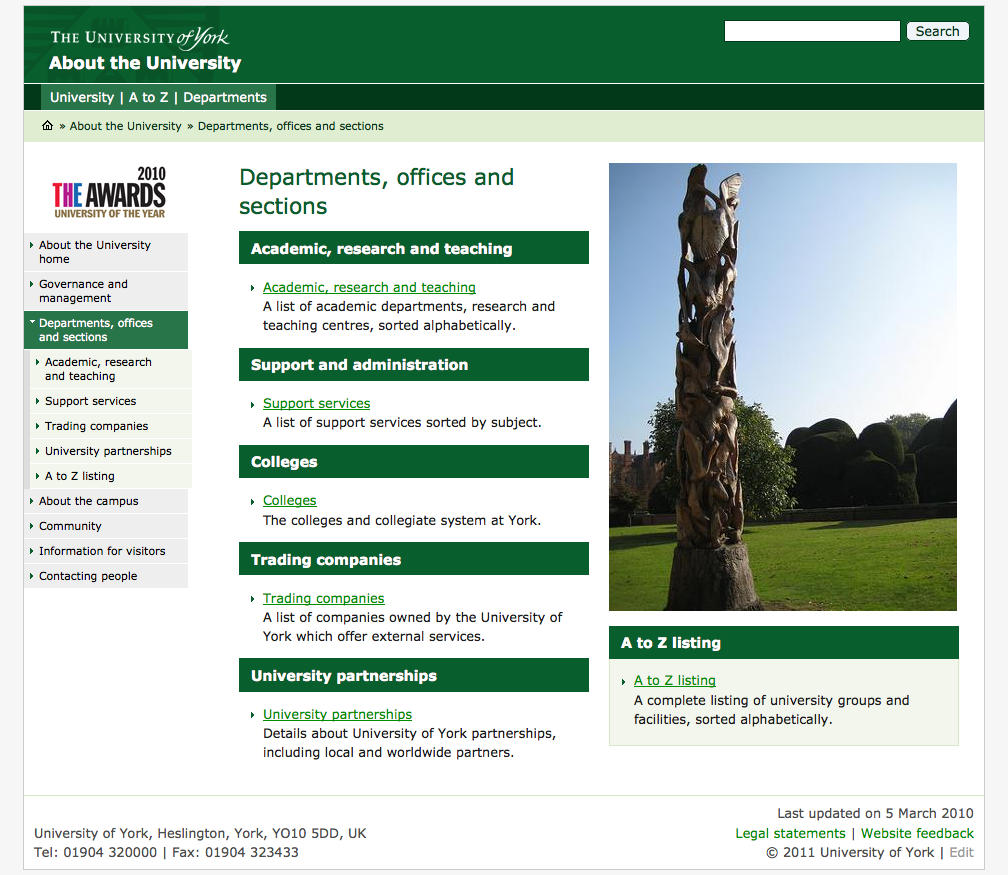
\includegraphics[width=160mm]{images/2011_11_06_yorkacuk.png}
  \end{center}
  \caption{A general page on the University site, using University colours.}
  \label{yorkacuk_general_page}
\end{figure}

\begin{figure}
  \begin{center}
    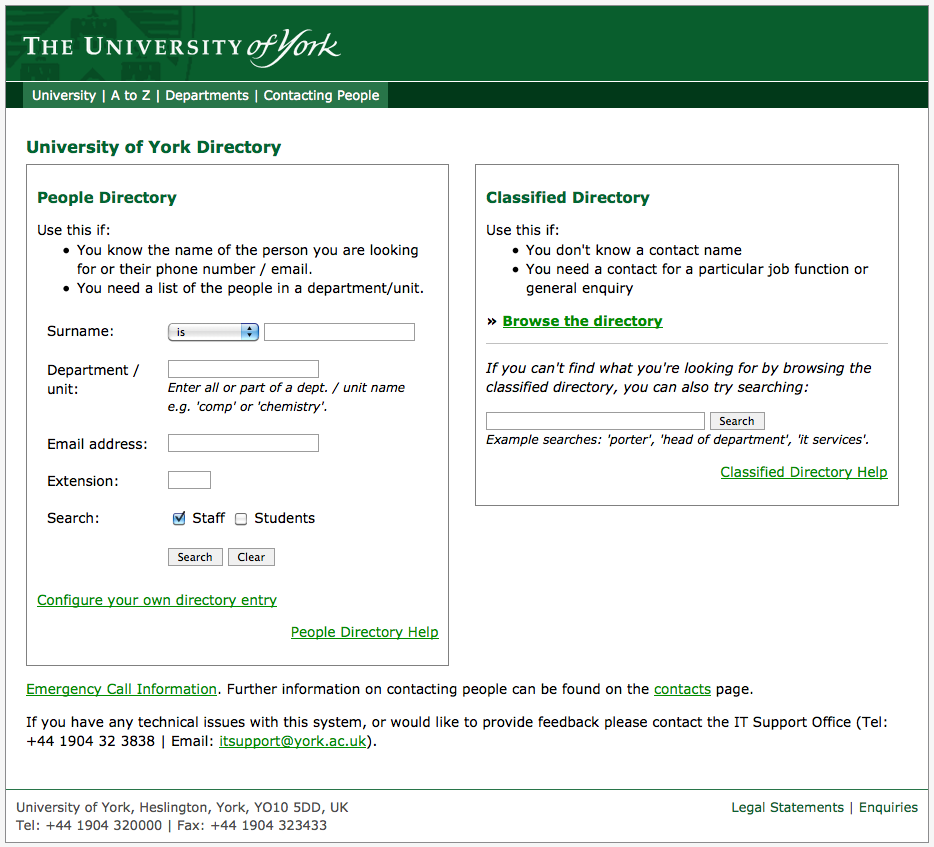
\includegraphics[width=160mm]{images/2011_11_06_yorkacuk_directory.png}
  \end{center}
  \caption{The University of York People Directory search tool.}
  \label{yorkacuk_directory_search}
\end{figure}

% Include screenshots of University software:
%   https://www.york.ac.uk/it-services/facilities/account/accounts
%   https://www.cs.york.ac.uk/submit/assessment/

One area that usability gains can be made are in relation to how the
application saves data. During one of the user research sessions, the
participant explained that while choosing optional modules during her first
year, she neglected to press that application's ``OK'' button and, unaware
that she had not submitted choices, was unable to take her preferred modules.

As an explicit ``Save'' button should be retained to reduce surprise and allow
the user to feel in control, the most sensible decision is to automatically
save user input periodically and notify users that their choices are being
saved. The submit button would save data in case of failure of the automatic
save mechanism.

\subsection{Accessibility}

Educational institutions such as the University of York are required by law to
ensure that web content is accessible to disabled users.

% http://www.york.ac.uk/communications/websites/policies/accessibility/
% http://www.york.ac.uk/communications/websites/content/accessibility/

The two major accessibility issues surrounding a web application are users who
are visually impaired and users who are unable to use a keyboard and/or mouse
to browse the web.

To mitigate the first accessibility issue, the application was tested to
ensure that users can increase the page or font size to fit their needs. Users
who use custom style sheets in their web browser (for example to enhance
contrast) are able to do so.

As to the second accessilibity issue, generally speaking users who are unable
to use a keyboard or mouse do not use JavaScript in their web browser. The
application is designed so that users with JavaScript disabled are instead
presented a simple form layout that can be read out to them and filled in with
the help of screen-reading software.

Finally, this application made use of the \texttt{<noscript>} HTML tag to
display the following to users who were attempting to choose their modules
with JavaScript disabled. Note that this text will also be read out by
screen-reading software.

\begin{quote}
  This page relies on JavaScript. If you're unable to use this application
  because of its dependence on JavaScript (for example, for accessibility
  reasons) please contact your departmental administrator for assistance.
\end{quote}

It is thought with these considerations, every student will be able to use the
system to select their modules. However, even if the above fallbacks fail the
student will still be able to obtain help from their department (which could
complete the module selection on their behalf). The aim is that no student
will be stranded with an application they cannot use and no instructions of
how to gain assistance.

\subsection{Interaction with other University software}

The system will be required to interact with \gls{sits}, as it is a centrally
maintained database that must always contain a true and accurate
representation of a student's data. Data stored in \gls{sits} is used in all
matters related to a student, including timetabling and room allocation.

This system will interact with \gls{sits} at two points:

\begin{enumerate}
  \item Module and student data must be imported during setup
  \item Student data must be exported after the allocation
\end{enumerate}

The import and setup will be performed by departmental administrators. This is
to reduce the workload on \gls{ssdt}, especially as administrators will be
required to tailor their setup after import.

For the pilot of this module allocation software, the export will be performed
manually by a member of \gls{ssdt}. They will perform a ``sanity check'' that
the data generated by this application seems accurate and will import the
data. If this application is evaluated successfully and maintained centrally,
it will not be feasible to import the data manually and some kind of automatic
import will have to be developed (Section~\ref{sec:autoexport}).

% Add notes from meeting with Matt

\subsection{Allocation algorithm}

During the research period, discussions with academic and administrative staff
in both pilot departments revealed that the current method of module
allocation is not particularly complex. With several hundred students in the
History department, it is impossible for a human to do a uniformly ``fair''
job of allocating modules to students. The staff simply try their best to
allocate as many high choices as possible.

With this information in hand, a score function was designed for the
constrained optimisation problem that also kept the module allocation system
as simple as possible.

One could imagine an imaginary score function that a staff member might have
in their head while allocating modules:

\begin{itemize}
  \item A first choice is perfect -- if every student received every one of
        their first choices, they would be happy.
  \item A second or third choice is alright -- a student would not be too
        displeased to be taking their second or third choice.
  \item A fourth or fifth choice should be avoided if possible, but is not a
        showstopper.
  \item One would expect a student who was being made to take their sixth or
        lower choice to be fairly unhappy.
\end{itemize}

Mathematically, one could sum a score for each student as follows:

$$
1(x_1) + 5(x_2) + 30(x_3) ...
$$

...where $x_i$ is the number of $i^{th}$ choices that that student was
allocated. The constant applied to the $i^{th}$ choice indicates a penalty
applied by the system -- this penalty increases depending on how negative that
choice is deemed to be.

While not particularly complex, one would expect that minimising this score
function would maximise the number of highly ranked choices.

The hard constraints on the optimisation problem are as follows:

\begin{itemize}
  \item The lower cap on a module (a module will not run if with less than the
        required number of students)
  \item The upper cap on a module (a staff member is not able to provide a
        certain quality of teaching to more than the maximum number of
        students)
  \item The number of credits a student must take from a particular group of
        modules (each student must have exactly the same workload as their
        peers)
\end{itemize}

The following constraints will be loaded into a constrained optimisation
solver and an allocation will be generated.

\subsection{Implementation schedule}

As the time allotted for implementation of the software was limited to under
eight weeks, it was necessary to prioritise certain aspects of the system in
case I was unable to implement every requirement.

Fortunately, the different elements of this project are naturally quite
loosely coupled. I identified the following aspects (ordered by priority):

\begin{enumerate}
  \item Student interface to collect data (27 Feb 2012)
  \item Performing the allocation (5 March 2012)
  \item Staff interface (approx 16 March 2012)
\end{enumerate}

The staff interface is given as the 16 March as it is not critical for this
pilot. While it would clearly be preferable for staff to set up the system
themselves unaided, it is more important that there is a working student
interface and allocation algorithm.

\subsection{Assistance provided with the application}

\subsubsection{Development work}

E.g. number of lines of code, type of code, time spent

% Code committed using a DVCS (Git) to GitHub so can easily see which commits
% came from which author

% So far: 2.5 hours

\subsubsection{Security review}

As the application is hosted by the University and will contain student data,
the project implementer met with the University's Information Security Officer
and one of the developers who assisted with the application code.

A review of the application architecture and code was conducted, and...
% echo $results

\subsection{Issues arising during implementation}

% Discuss some of the _real_ issues of a _real_ project

\noindent{\textbf{Availability of stakeholders}}

One of the most positive aspects of undertaking this project was in fact one
of the most difficult -- that is, the project was designed to work very
closely with the University of York and as such relied on ``real''
stakeholders.

An issue arose fairly early in the project when it became clear that some
administrative staff (both IT support staff and those in the pilot
departments) would be away from work for prolonged periods of time or would
leaving their jobs during the creation of this application. This caused delays
while the replacement staff had to be brought up to speed on the background
and current state of the project.

The issue was mitigated with the help of the \gls{aso}, which was responsible
for assisting with issues not directly related to implementation. The new or
replacement staff were then invited to group meetings so that they could keep
up to speed with recent developments and provide any necessary input. As
implementation began to finish, departmental administrators were provided
training on the software by the project implementer. A deputy was present at
the training sessions so that the software could still be used in case of
unforeseen circumstances rendering the departmental administrator unable to
set up the software.

% \noindent{\textbf{Lack of technical contacts available during the project}}

% Discuss how no technical people were involved early enough.

% \noindent{\textbf{Inability to interact with the system while it contained sensitive data}}

% I was unable to respond to bugs in a timely manner as I couldn't have access
% to student data.

% The University explored whether the project implementer could sign a
% non-disclosure agreement with regards to the student data involved in the
% system.

\noindent{\textbf{Unfamiliarity with the language and framework}}

While the framework was chosen based on its maintainability as
University-owned software, the project implementer was not particularly
familiar with the underlying language and framework. This made it hard to
estimate the amount of time that various stages of implementation would take.
If this project was to be undertaken again, the implementer should first use a
language they are familiar with to prototype the application quickly, and then
use any remaining time to re-implement in a language that can be maintained by
the future software owners.

This would require almost double the implementation effort (though parts, such
as the user experience and some front-end code, could be reused across
frameworks) but should allow the implementer to provide clients with a working
application far in advance of any deadlines. When developing using unfamiliar
software, the developer is dependent on how fast they are able to learn and
use new techniques.

\subsection{Testing}

How will the software be tested?

\subsection{Pilot by the Archaeology and History departments}

During the spring term, the Archaeology and History departments at the
University of York used this application to allocate modules to their
second-year students.

% Departmental administrators in both departments set up the application
% during the week commencing 20 February 2012, and students used the
% application to select their modules between 27 February and 7 March.
% 
% As the application was hosted by \gls{itservices}, documentation was created
% in advance and provided to the team that provides end-user support. Issues
% were logged from emails to \texttt{itsupport@york.ac.uk}, telephone calls
% and visits to the IT Support office. A summary of these issues is provided
% in (appendix x).

\section{Further work}
\label{sec:furtherwork}

% A chapter describing possible ways in which your work could be continued or
% developed. Be imaginative but realistic.

We should probably ask departments what they'd like to see in the future.

There were many feature requests from the pilot departments that I had
insufficient time to implement during the course of the project.

\subsection{Maintaining a history}

While considering the data protection implications mentioned in
Section~\ref{sec:dataprotection}, a popular request from the pilot departments
was that the application should retain its knowledge about a student for the
duration of their time at university.

One obvious benefit of this improvement is that the allocation could be made
more fair over the course of a student's academic career. For example, if a
student was given one of their lower ranked modules in their first year, the
allocation could compensate them by giving them preference for a higher ranked
module in their second year.

The University's Data Protection Officer would have to be consulted in order
to draft a suitable retention policy for this additional data. It seems that
this is data a department might be expected to collect and reference, and as
such could be held in line with the department's retention policies.

\subsection{Different methods of obtaining information from students}

If I didn't have time to implement a weighting system (rather than a simple,
plain ranking system) I could talk about that here.

One mockup created during the user testing allowed students to weight modules
rather than ranking them -- it was thought by the project steering group that
this interface (Figure~\ref{prototype_student_weighting}) would allow students
to express more clearly their preferences for certain modules (i.e. the
student could use the bars to demonstrate that they have a strong desire for
module X, and absolutely do not want to be allocated module Y).

However, during user testing the students were confused about how the values
shown on the bars would be used to allocate modules. There was strong feedback
from the test groups that the application should in fact be kept as simple as
possible -- the phrase \gls{kiss} is often used.

It is possible that an interface similar to the one prototyped could be
further refined such that students are comfortable using it -- the project
group and implementer still believe it could provide a ``better'' allocation
for students, though perhaps not in its current form.

\subsection{Automatic import and export}
\label{sec:autoexport}

The application could automatically import and export data.

\subsection{Expanding the use of the application}

The Chair of Board of Studies in Archaeology posed the question of whether
this application could be used to allow visiting students to select their
modules.

\subsection{Interface improvements}

As departments have different requirements for the algorithm, it would be nice
if they could manipulate (nuances) in the algorithm themselves.

The student interface should be improved so that it functions properly on
devices that accept different forms of user input. This was deemed unimportant
for the pilot project as the application was only accessible from campus PCs
or using the University's \gls{vpn}. However, if the application was available
on the web, it is increasingly likely that students would attempt to use
touchscreen devices to access the application. Further testing should be
conducted using common examples of such devices and any outstanding issues
should be fixed.

\section{Conclusions}
\label{sec:conclusions}

% This is similar to the abstract. The difference is that you should assume
% here that the reader of the conclusions has read the rest of the report.

While the research carried out formed a strong basis for a web application,
the lack of time to implement meant that some parts of the research could not
be considered fully for this particular application.

\appendix

% What should go in an appendix? Screenshots? Code? Something else?

\clearpage
\section{External links}

This appendix gives URLs to departments, offices or services mentioned
throughout the document.

University Teaching Committee sponsored this project on behalf of the
University of York:
\url{http://www.york.ac.uk/about/organisation/governance/sub-committees/teaching-committee/}

IT Services hosted and maintained the application once it had been created:
\url{http://www.york.ac.uk/it-services/}

I would like to make the code of this software available online, at
\url{https://github.com/alexmuller/york-allocation}.

\clearpage
\section{Participant consent form}
\label{sec:consent}

All research participants (students and staff of the University of York)
signed the consent form shown in Figure~\ref{participantconsent} immediately
before their interview took place. This consent form is adapted from one made
available by Alistair Edwards for Computer Science students to use during
their projects. As of 5 November 2011, the original is available at
\url{http://www-users.cs.york.ac.uk/~alistair/projects/consent.html}.

In each case, the top half of the form was retained by the project author and
the second half was given to the participant in case they had any further
questions about the interview.

\begin{figure}[h]
  \begin{center}
    \fbox{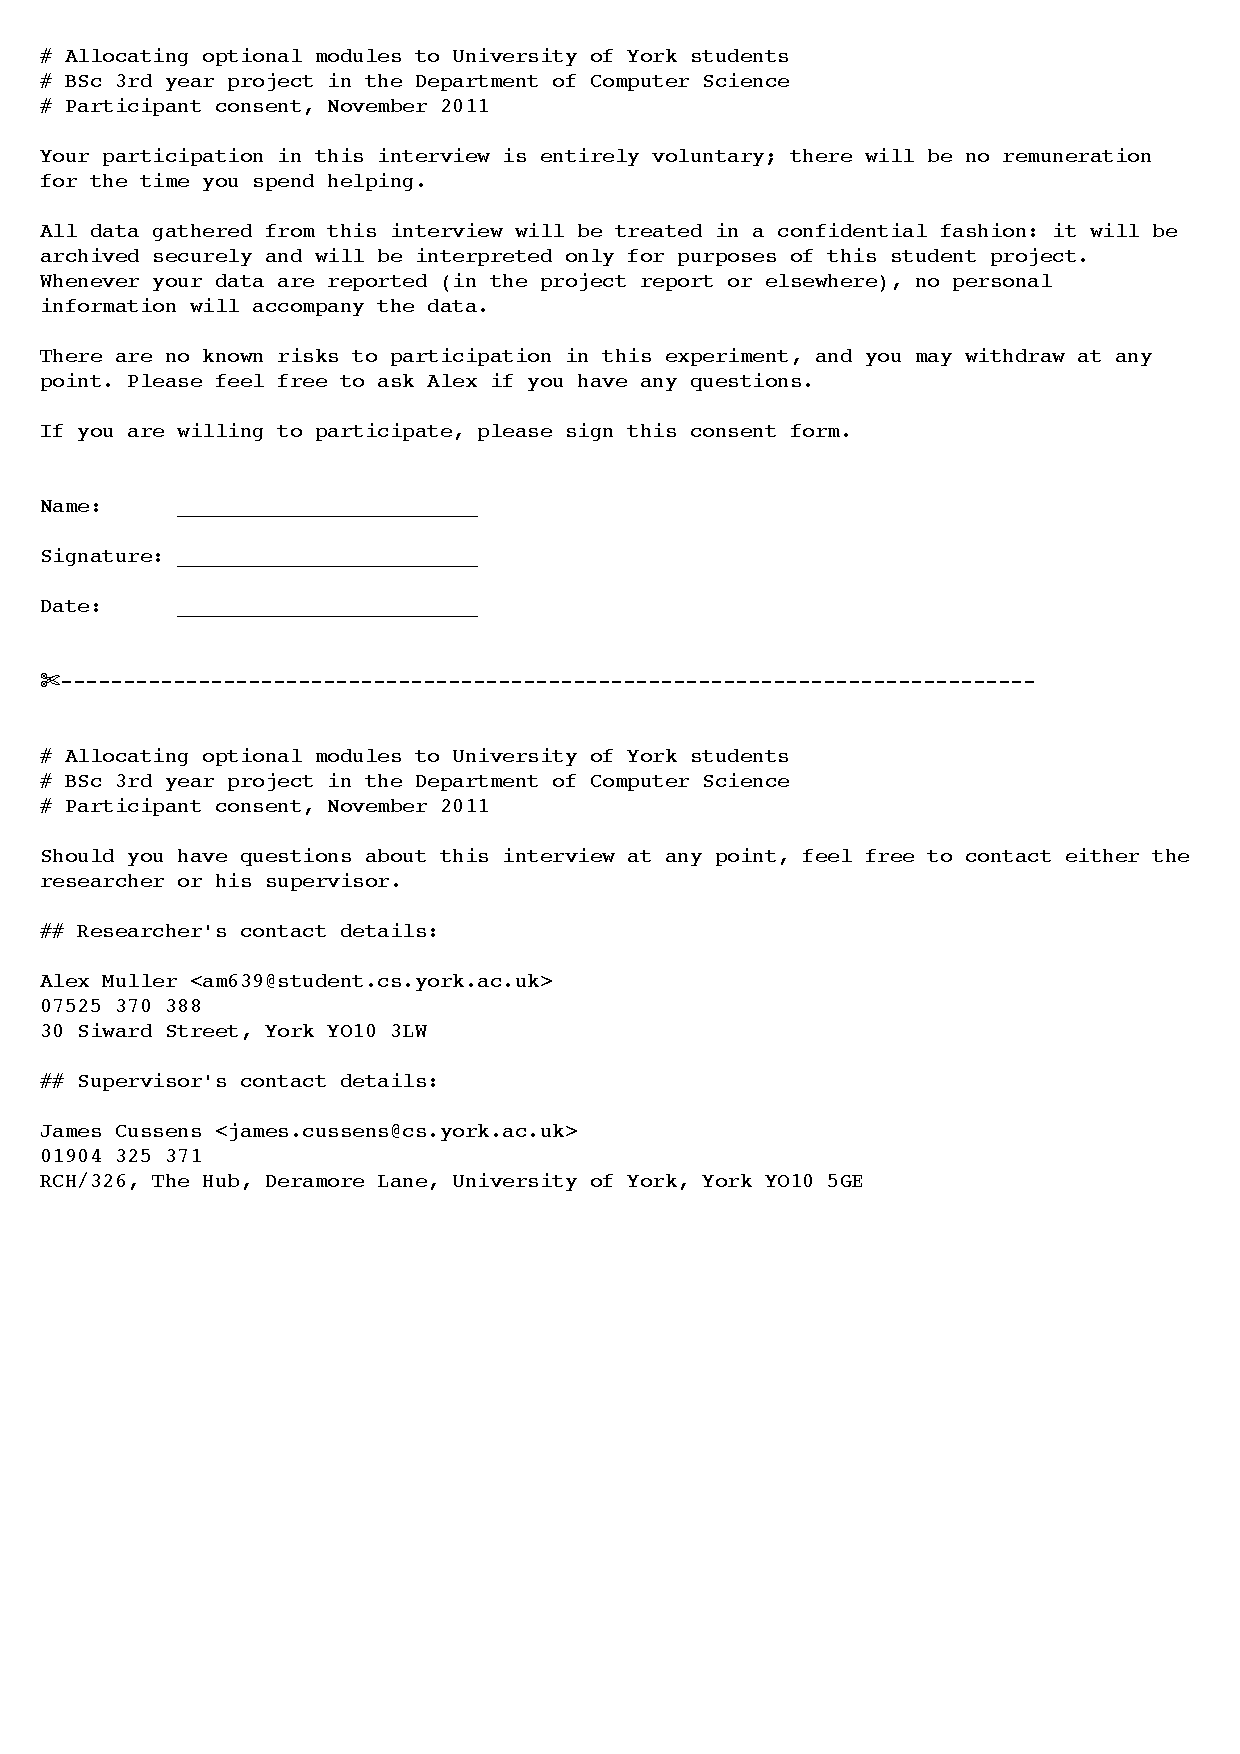
\includegraphics[width=0.9\linewidth, trim=0 80mm 0 0]{images/consent.pdf}}
  \end{center}
  \caption{Participant consent form.}
  \label{participantconsent}
\end{figure}

\clearpage
\section{Prototypes of the student interface}
\label{sec:prototypes}

This appendix gives screenshots of the prototypes created for the student
interface for ranking modules.

Note that the explanatory copy included in the screenshots below was drafted
by the project implementer and was revised by the departments prior to the
system being in use.

\begin{figure}[h]
  \begin{center}
    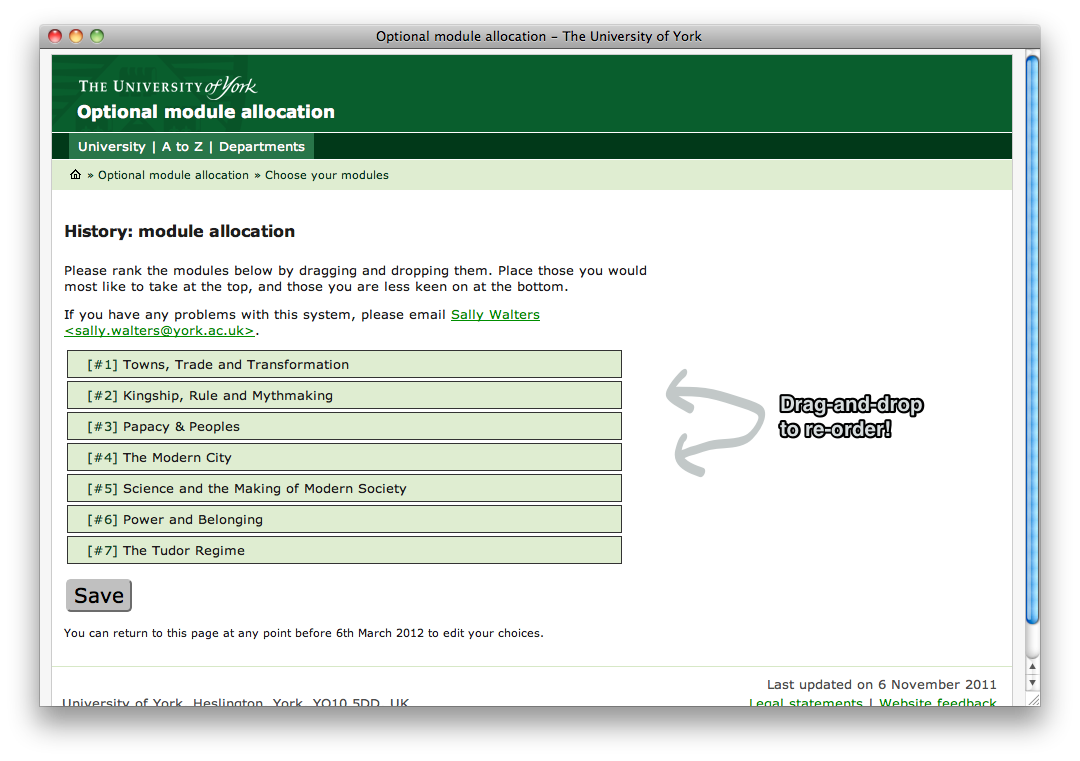
\includegraphics[width=0.85\linewidth]{images/prototypes/student_prototype_1.png}
  \end{center}
  \caption{Prototype of a drag-and-drop ranking based system}
\end{figure}

\begin{figure}
  \begin{center}
    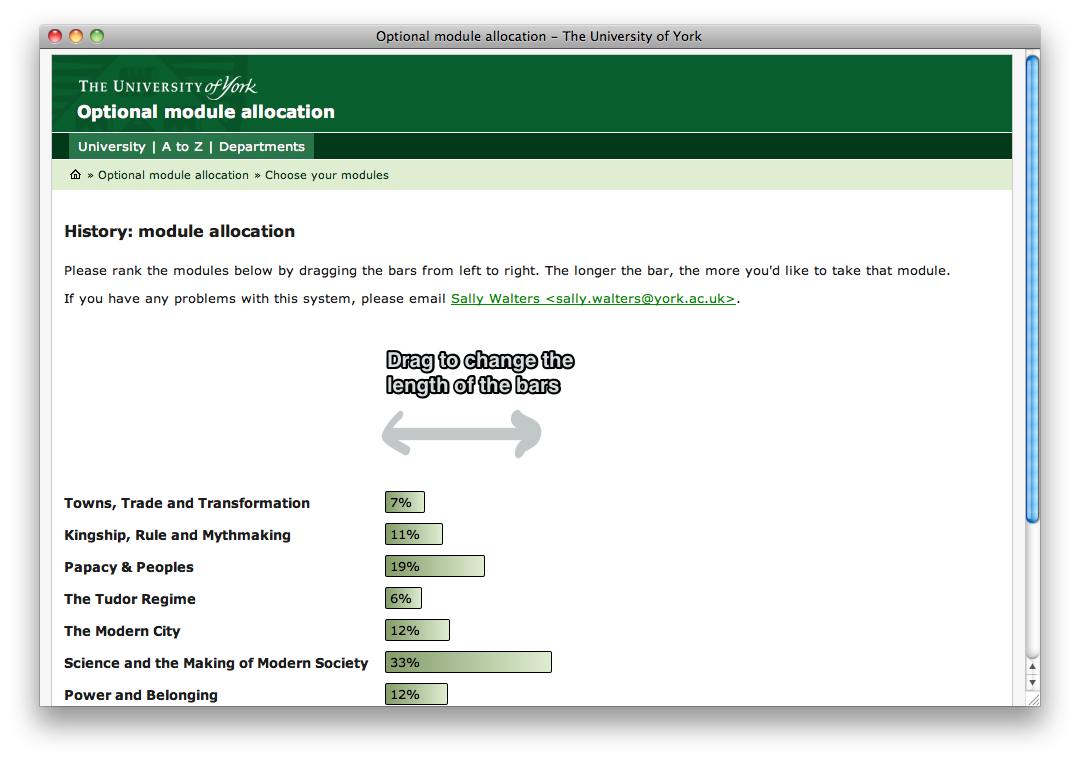
\includegraphics[width=0.85\linewidth]{images/prototypes/student_prototype_2.png}
  \end{center}
  \caption{Prototype of draggable bars for a weighting based system}
  \label{prototype_student_weighting}
\end{figure}

\begin{figure}
  \begin{center}
    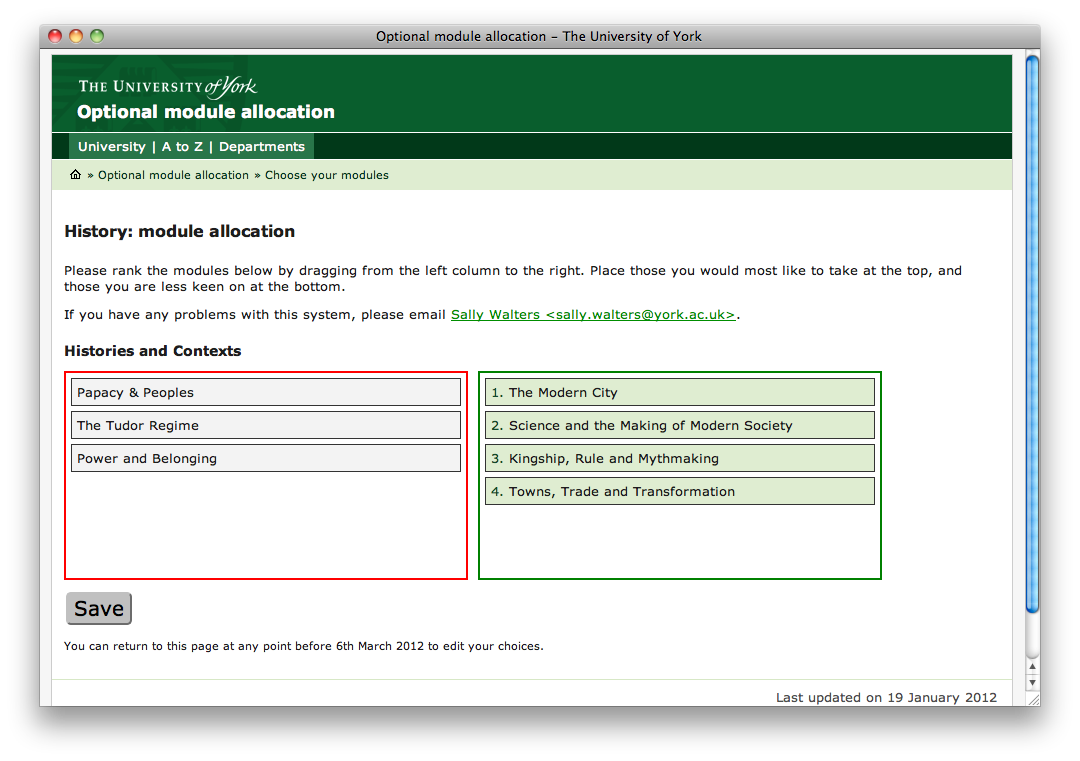
\includegraphics[width=0.85\linewidth]{images/prototypes/student_prototype_3.png}
  \end{center}
  \caption{Prototype of a drag-and-drop two-column ranking based system}
  \label{prototype_student_2col}
\end{figure}

\clearpage
\printglossaries

\clearpage
\bibliographystyle{references/IEEEtran.bst} % not just plain
\bibliography{references/references.bib}


\end{document}
